\documentclass[tikz,border=10pt]{standalone}
% No extra libraries needed
\begin{document}
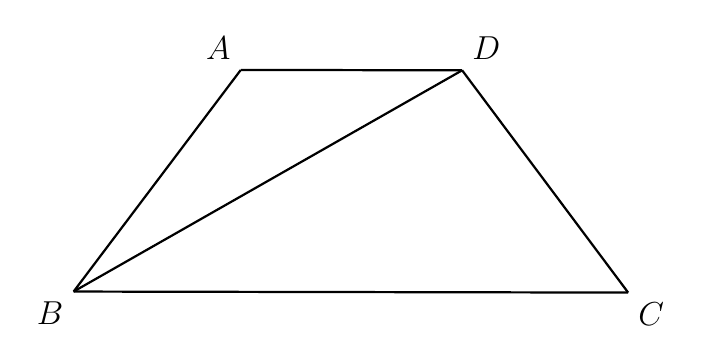
\begin{tikzpicture}[line join=round, line width=0.8pt]
  % Vertices (pixel -> cm, s = 0.014953, y flipped)
  \coordinate (A) at (-1.390595256129746,1.4230821935945894);
  \coordinate (D) at (1.4204952561297457,1.4179178064054108);
  \coordinate (C) at (3.528901893484577,-1.4045693337860679);
  \coordinate (B) at (-3.513901893484577,-1.3916306662139322);

  % Edges: top AD, bottom BC, left AB, right CD, diagonal BD
  \draw (A) -- (D);
  \draw (B) -- (C);
  \draw (A) -- (B);
  \draw (C) -- (D);
  \draw (B) -- (D);

  % Labels just outside each vertex
  \node[above left] at (A) {\fontsize{12}{14.4}\selectfont $A$};
  \node[above right] at (D) {\fontsize{12}{14.4}\selectfont $D$};
  \node[below right] at (C) {\fontsize{12}{14.4}\selectfont $C$};
  \node[below left] at (B) {\fontsize{12}{14.4}\selectfont $B$};
\end{tikzpicture}
\end{document}